\documentclass[11pt]{article}
\usepackage[textheight=9in]{geometry}
\usepackage{graphicx}
\usepackage{epstopdf}
\usepackage{listings}
\usepackage{float}
\usepackage{wrapfig}
\usepackage{fancyref}
\usepackage{upquote}
\usepackage{scrextend}
\usepackage{csquotes}
\usepackage[font=small,labelfont=small]{caption}
\usepackage{mdframed}
\usepackage{hyperref}

\hypersetup{
	colorlinks=true,
	urlcolor=blue
}

\def\f{Fig.}
\def\s{Sec.}
\def\l{Listing}
\def\e{Eq.}

\def\emw{7.5mm}
\lstset{language=TeX,tabsize=2,basicstyle=\footnotesize\ttfamily,xleftmargin=\emw,xrightmargin=\emw}
\setlength{\parindent}{0em}

\title{Cyclicity User Manual}
\author{Emily Schlafly and Yuliy Baryshnikov}
\date{Spring 2016}

\begin{document}

\maketitle

{\hypersetup{linkcolor=black}
\tableofcontents
}

\setlength{\parskip}{1em}

\pagebreak

\begin{mdframed}
\section{Quickstart}

These are the basic functions you will work with. Start by downloading the \href{https://uofi.box.com/s/k3wci00baw39axgz3070c8325ej601io}{sample data} to the \textit{data} folder in the \textit{cyclicity} folder. In Matlab, navigate to the \textit{cyclicity} folder and enter the following: 

\lstinputlisting{../cyclicity/quickstart.m}

What follows is an explanation of what each of the functions do and how to use them. Additionally, you can use the \verb|help| command in Matlab to see function usage.

\end{mdframed}

\pagebreak

\section{Introduction}
\input{sectionIntroduction}

\section{Toy Data Examples}
\input{sectionToyExamples}

\section{fMRI Examples}
\input{sectionFMRIexamples}

\section{Looking at Results}
This section is meant to address the issue of how to compare and contrast the cyclicity results across subjects and how to interpret results on the whole. The first metric that we look at is the eigenvalue ratios which gives us an idea of the quality of analysis. The other three metrics that we look at are different ways of looking for consistencies in the data.

\subsection{Eigenvalue Ratios}

\begin{lstlisting}[frame=single]
eval_ratio = evalRatio(dir_search, outid, exp_setup);
\end{lstlisting}

When considering the quality of the cyclicity results, we look for the ratio between the magnitude of the first eigenvalue pair and that of the second eigenvalue pair to be greater than two. Ratios at or around two are what we would find if the trajectories were completely unrelated brownian motions so we want to see that the data have a more clear relationship than random trajectories.

Let's start by looking at random data:

\begin{figure}[H]
\begin{minipage}{.6\linewidth}
\begin{lstlisting}
brownian = arrayfun(@(x) ...
	createToy('brownian','time',1000),	...
	(1:100),'UniformOutput',0);
output = analyzeCyclicity(brownian);
ratios = evalRatio(output);
\end{lstlisting}
\end{minipage}
\hfill
\begin{minipage}{.39\linewidth}
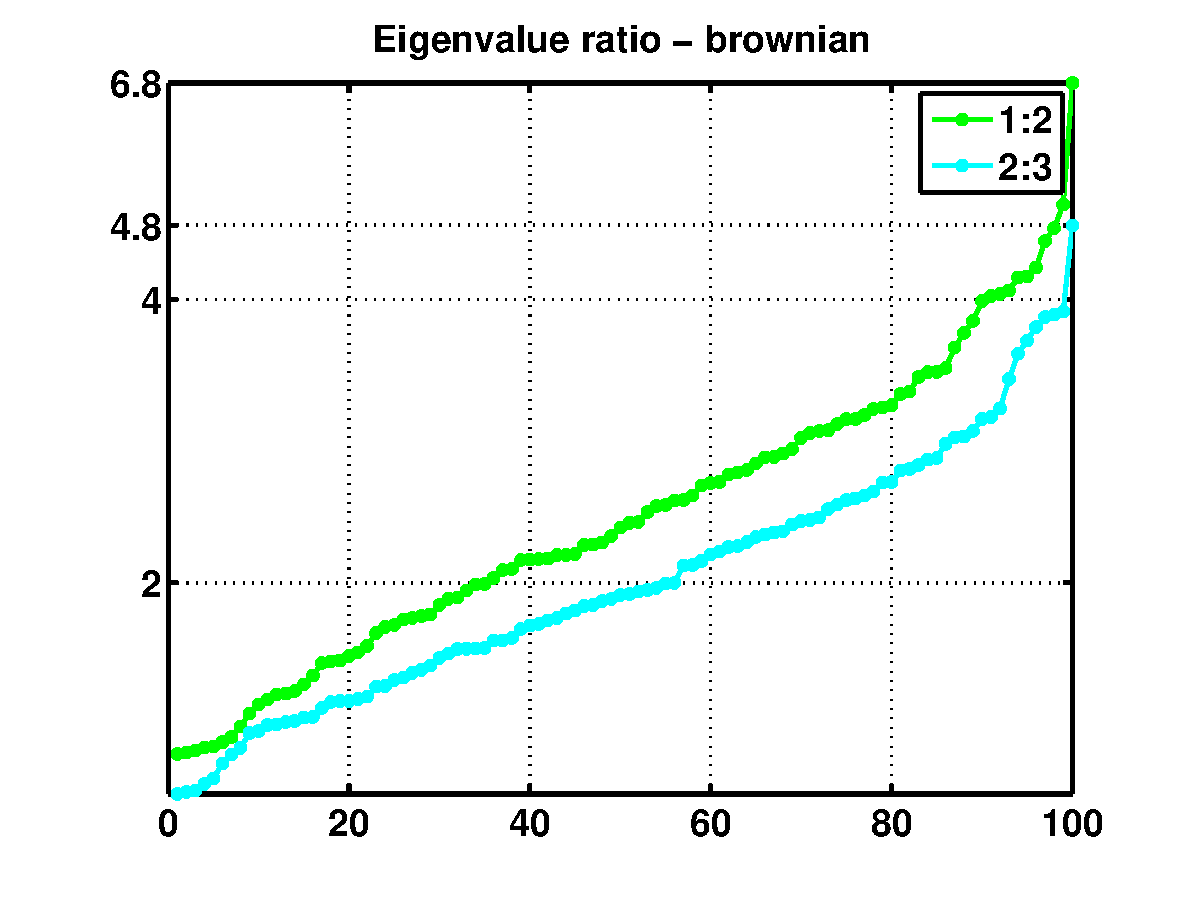
\includegraphics[width=\linewidth]{figs/brownian_evalRatio.eps}
\end{minipage}
\caption{Eigenvalue ratios of brownian motion. Notice how the first and second ratios run parallel to each other and 90\% of the ratios are less than 4. We need our data to have higher ratios than shown here, with more differentiation between the first (1:2) and second (2:3) ratios.}
\label{fig:brownian}
\end{figure}

In order for our results to be meaningful, we need to see a plot that looks different from the one above. So now let's look at some results that we got from subjects that we analyzed from the Human Connectome Project.

\begin{figure}[H]
\begin{minipage}{.6\linewidth}
\begin{lstlisting}
ratios = evalRatio('cyclicityHCP.mat');
\end{lstlisting}
\end{minipage}
\hfill
\begin{minipage}{.39\linewidth}
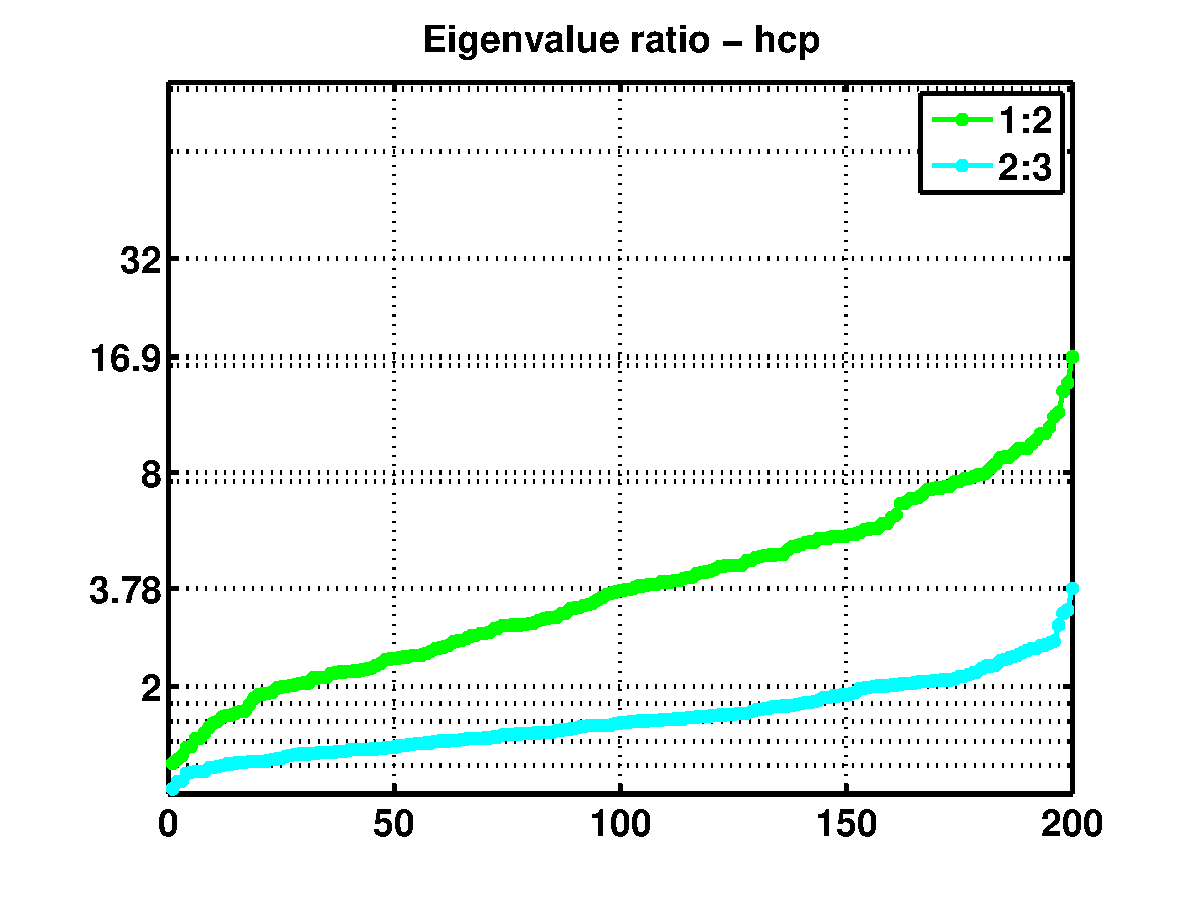
\includegraphics[width=\linewidth]{figs/hcp_evalRatio.eps}
\end{minipage}
\caption{Eigenvalue ratios of HCP subjects. Approximately 40\% of subjects have eigenvalue ratios over 4 and the second ratio stays much lower with more than 80\% of the ratios less than 2 as compared to only about 50\% less than 2 in the brownian case.}
\label{fig:hcpevals}
\end{figure}

In the legend, `1:2' (`2:3') refers to the magnitude of the first (second) pair of eigenvalues to that of the second (third) pair of eigenvalues. We look at this plot in order to determine if we are actually picking up on any real signal, rather than randomness. In the long time limit, the eigenvalue ratios of brownian motion lead matrices approach 2, but in general our data sets are only about 1000 time steps long, so we should get an idea for how a random data set would look in this time frame. Looking at the plot of the eigenvalue ratios for the brownian motion trajectories (\f~\ref{fig:brownian}), about 90\% of the 1:2 ratios are below 4 and about 50\% of the 2:3 ratios are below 2, and additionally, the 1:2 and 2:3 ratios run approximately parallel to each other. 

In \f~\ref{fig:hcpevals}, on the other hand, we see the eigenvalue ratios for fMRI data from the Human Connectome Project (HCP). There are a few differences between \f~\ref{fig:brownian} and \f~\ref{fig:hcpevals} which lead us to the conclusion that this method is picking up on an interesting signal: 1.) the 1:2 ratios are, in general, much higher - only about 50\% of these are less than 4 compared with about 90\% in \f~\ref{fig:brownian}, 2.) about 75\% of the 2:3 ratios are less than 2 (compared with approximately 50\%), and 3.) the 1:2 and 2:3 ratios do not run parallel to each other as in the brownian motion analysis. 

One approach that we have not pursued, but might be worth investigating is to weed out subjects with low eigenvalue ratios and then do the group analyses described below.

\subsection{Order Distribution}

\begin{lstlisting}[frame=single]
perm_locs = permLocations(dir_search, numClusters, outid, ...
	region_names, exp_setup)
\end{lstlisting}

One analysis that we were able to get some interesting insight from was where in the permutation a given region appeared. At one point we narrowed our regions down to those that had the strongest signal across all subjects from the HCP data set and what we saw was that the left primary auditory cortex was consistenly showing up very early in the permutation sequence. I never found a way to visualize this that I was completely happy with, so there are a few plots for this one.

\newcommand\w{.49}
\begin{figure}
\begin{lstlisting}
pl = permLocations('cyclicityHCP.mat',5);
\end{lstlisting}
\includegraphics[width=\w\linewidth]{figs/cyclicityHCP_permLocationsstd.eps}
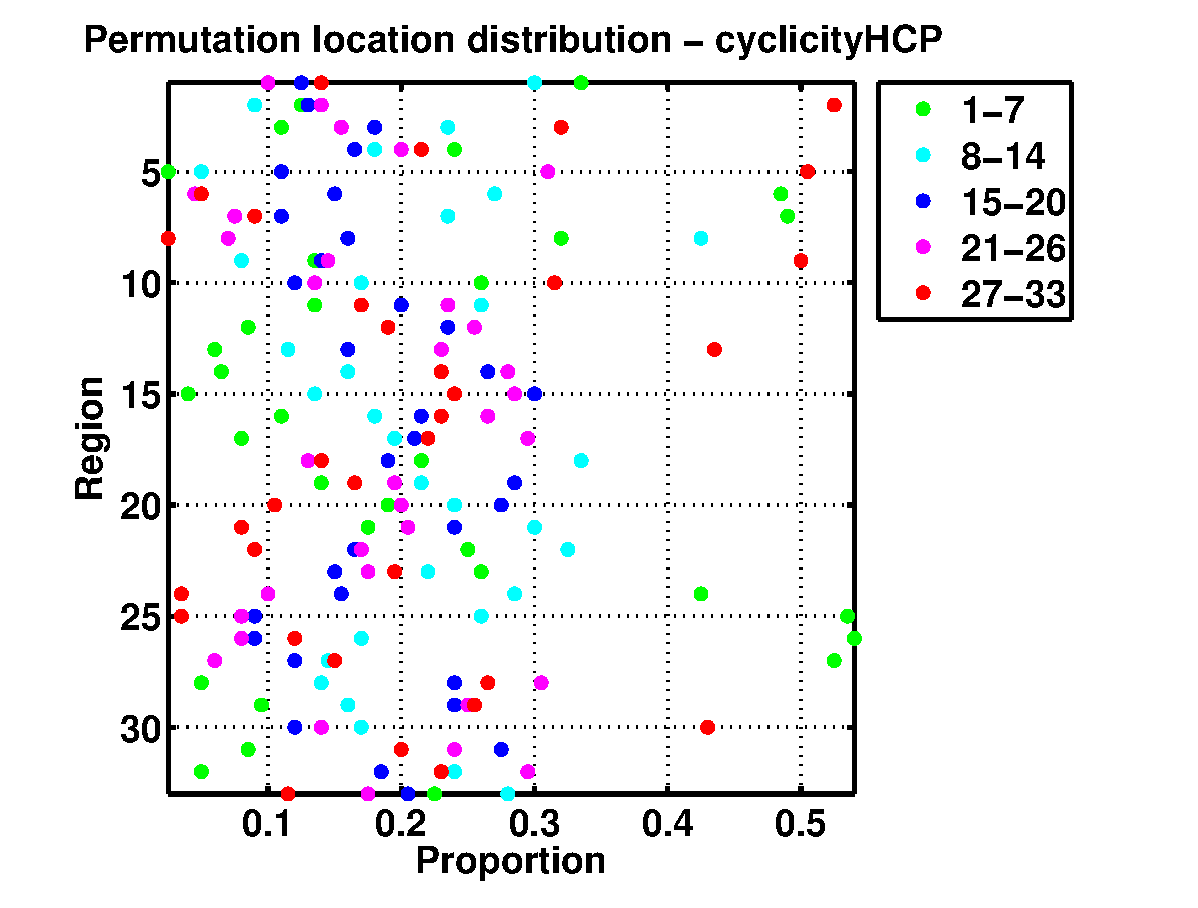
\includegraphics[width=\w\linewidth]{figs/cyclicityHCP_permLocationsdots.eps}
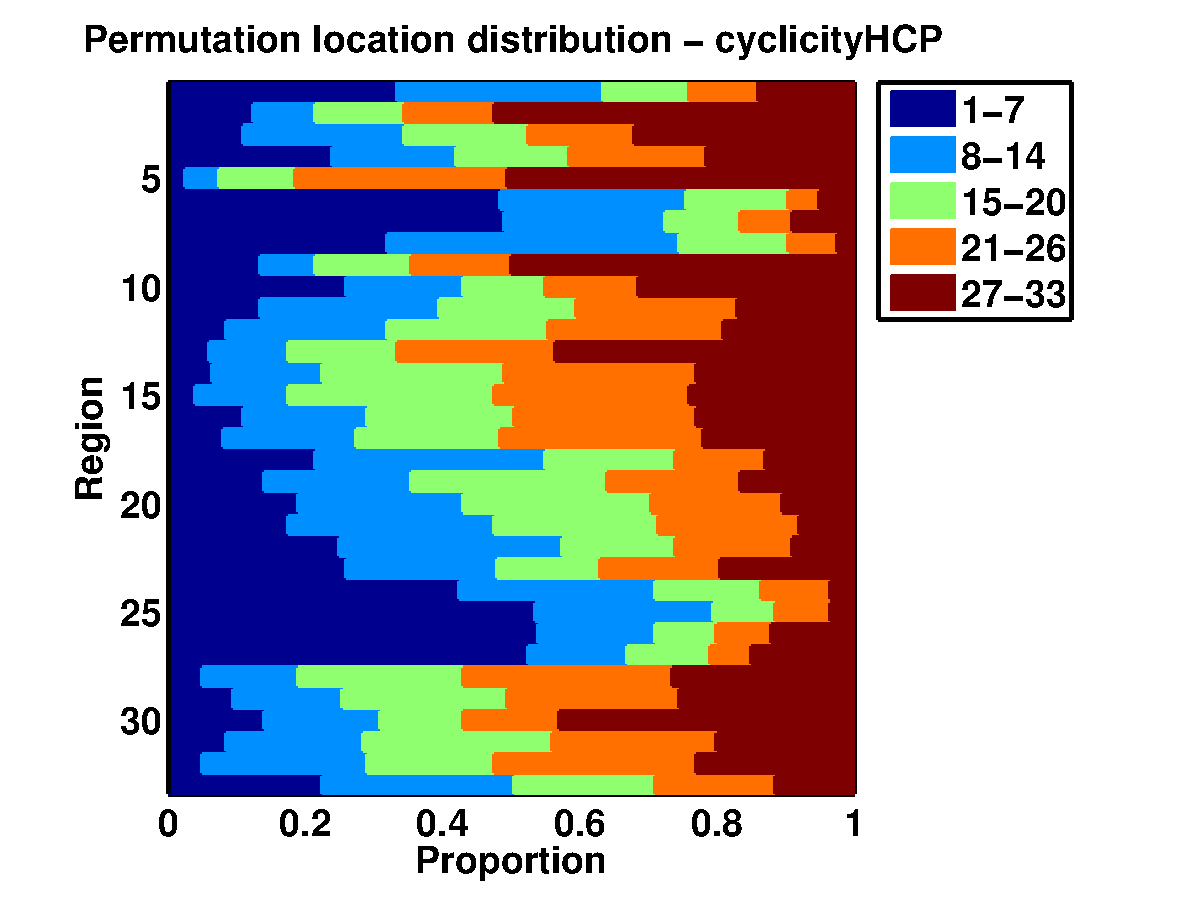
\includegraphics[width=\w\linewidth]{figs/cyclicityHCP_permLocationsbars.eps}
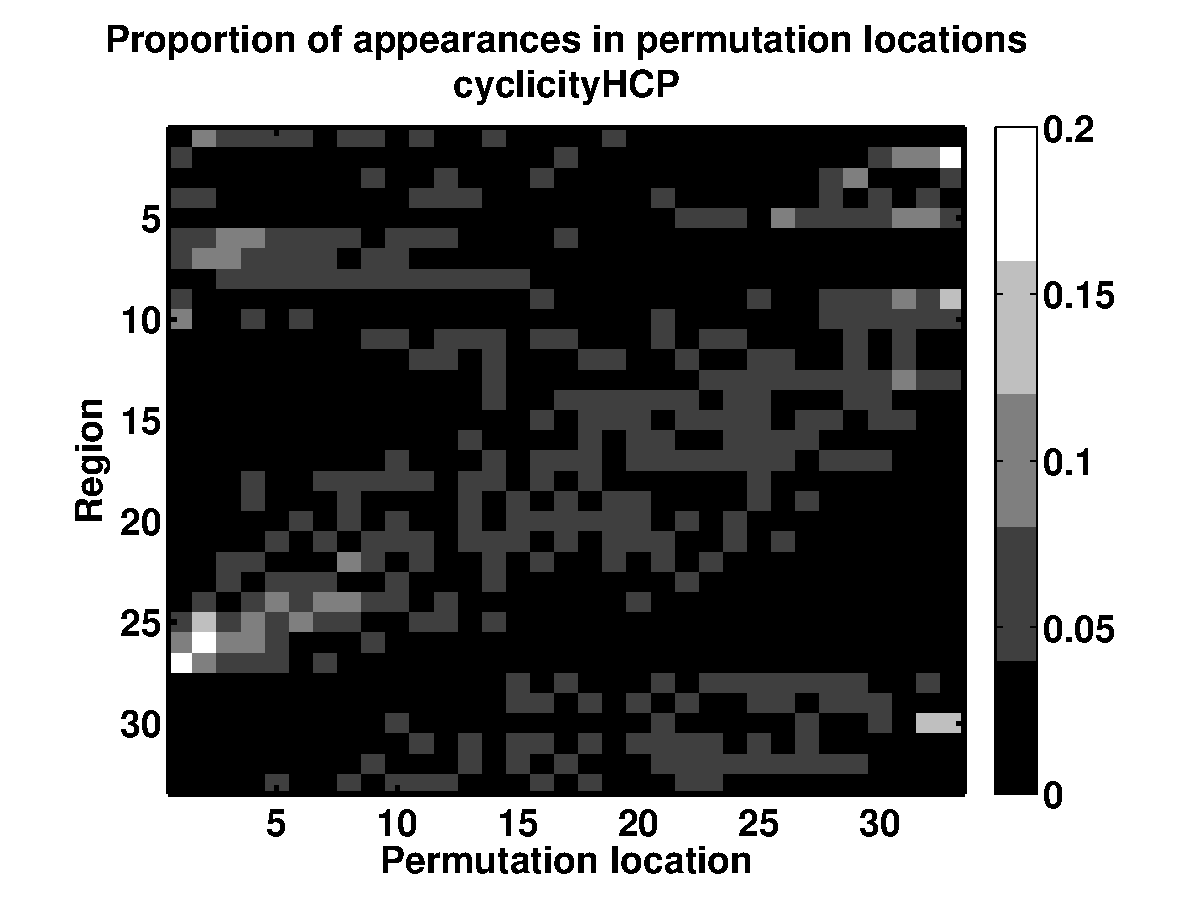
\includegraphics[width=\w\linewidth]{figs/cyclicityHCP_permLocationsgray.eps}
\caption{(top left) This plot shows the standard deviation for each region. Regions that stay clustered around one location will have a higher standard deviation than those that are more evenly distributed across locations. (top right) The benefit to this style is that it is very easy to see outliers and approximately where in the permutation they sit. The down side this divides the permutation locations into the number of regions indicated so the location of the cutoff will affect how this plot looks. (bottom left) This is a bar plot of the same values as in the top right plot - no new information, but easier to see the distribution for a certain region. (bottom right) This shows the proportion of times the region appeared in each permutation location. This plot and the top left in combination are probably the most useful.}
\label{fig:permLocations}
\end{figure}

The top left plot in \f~\ref{fig:permLocations} shows the standard deviation of the proportion of time spent in each location for each region. A higher standard deviation means that a region concentrates in only a few locations in the permutation so higher values are more interesting here. The plot in the lower right shows the proportion of subjects in which each region appears in each location. Using this plot in combination with the plot in the upper left corner highlights which regions are more localized and where they are found. 

The other two plots give two different views of the same thing. They show the proportion of times each region shows up in a subset of locations. For example, the top right plot says that region 2 was in permutation location 27-33 more than 50\% of the time and region 25 was in location 1-7 about 55\% of the time. The number of subsets is given by the second input value and the locations are split as evenly as can be (favoring the beginning and ending subsets - the first and last groups have 7 locations, while the middle group has only 6).

Alternatively, use the following to show the region names and export the figure to an .eps file:

\begin{lstlisting}
pl = permLocations('cyclicityHCP.mat',5,[],'rois.mat','eps');
\end{lstlisting}

\subsection{Signal Champions}

\begin{lstlisting}[frame=single]
[regions,counts] = phaseHist(dir_search, top_n, outid, ...
	region_names, exp_setup)
\end{lstlisting}

The signal champions are the regions that consistently have a high absolute values across subjects. The \verb|phaseHist| function makes a histogram of the regions which have phase magnitudes in the top \verb|top_n| for each subject. The higher signal indicates a more clear placement in the permutation, so these should be regions for which the algorithm works well.

\begin{figure}
\begin{minipage}{.55\linewidth}
\begin{lstlisting}
[regions,counts] = ...
	phaseHist('cyclicityHCP.mat');
\end{lstlisting}
\end{minipage}
\hfill
\begin{minipage}{.45\linewidth}
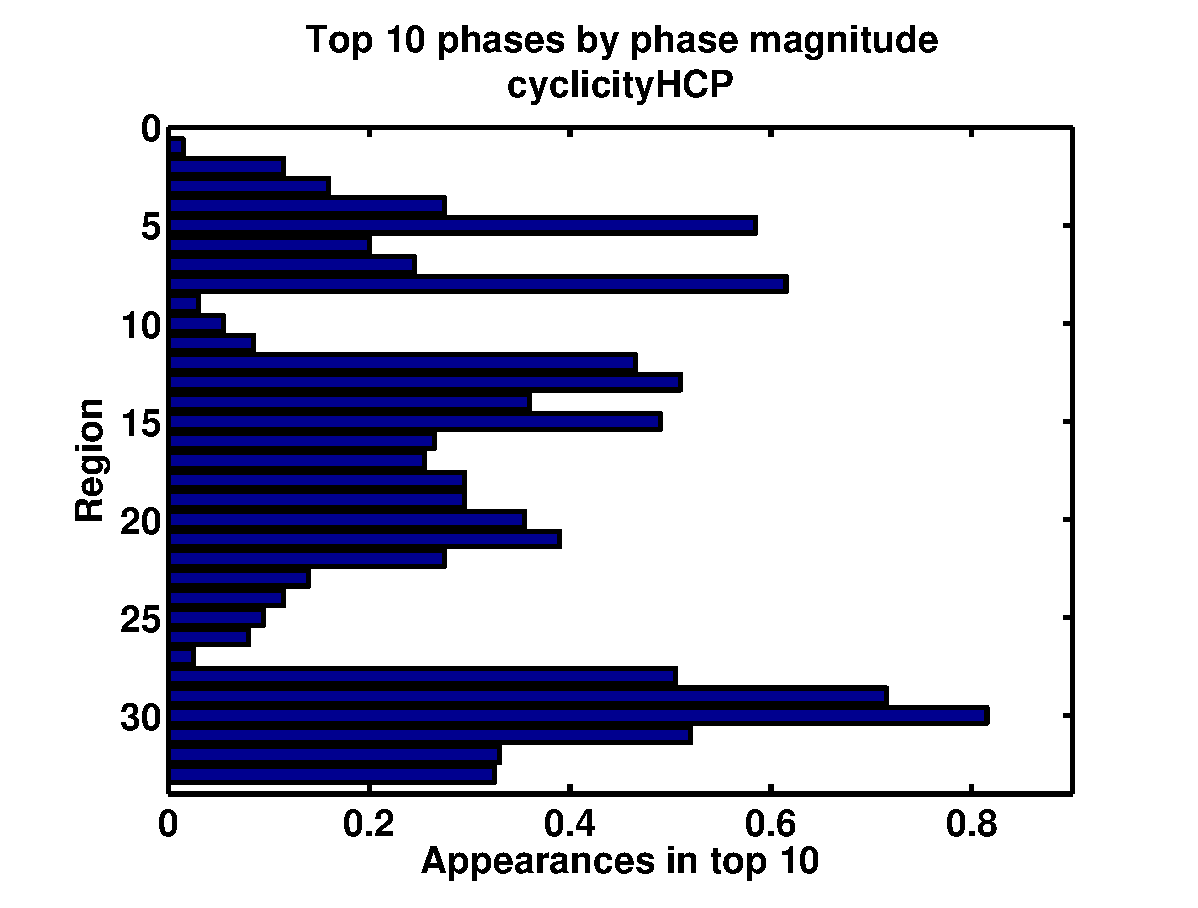
\includegraphics[width=\linewidth]{figs/phaseHist.eps}
\end{minipage}
\caption{Histogram of regions with phase magnitudes in top 10 for each subject. Looking at this plot, we would conclude that the algorithm works well for regions 5, 8, 29, and 30 so from here, we might decide to focus on these regions.}
\end{figure}

\subsection{Triples}

\begin{lstlisting}[frame=single]
trips = makeTriples(dir_search, thresh, outid, region_names, ...
    exp_setup)
\end{lstlisting}

This function will return all triples which appear in at least \verb|thresh| proportion of subjects, where \verb|thresh| is in $[0,1].$ It will also save a text file with the results. If \verb|dir_search| is a cell or regular expression matching multiple files then it will also display a plot comparing which triples appear at or above the given threshold for each data set. \f~\ref{fig:makeTriples} shows triples from cyclicity results from a group with normal hearing and a group with tinnitus (\textit{NH\_cyclicity.mat} and \textit{TIN\_cyclicity.mat}, respectively).

\begin{figure}
\begin{minipage}{\linewidth}
\begin{lstlisting}
trips = makeTriples('*_cyclicity.mat', .8, [], 'rois.mat'); 
% or equivalently
trips = makeTriples({'NH_cyclicity.mat';'TIN_cyclicity.mat'}, .8, ...
	[], 'rois.mat'); 	
\end{lstlisting}
\end{minipage}
\hfill
\begin{minipage}{\linewidth}
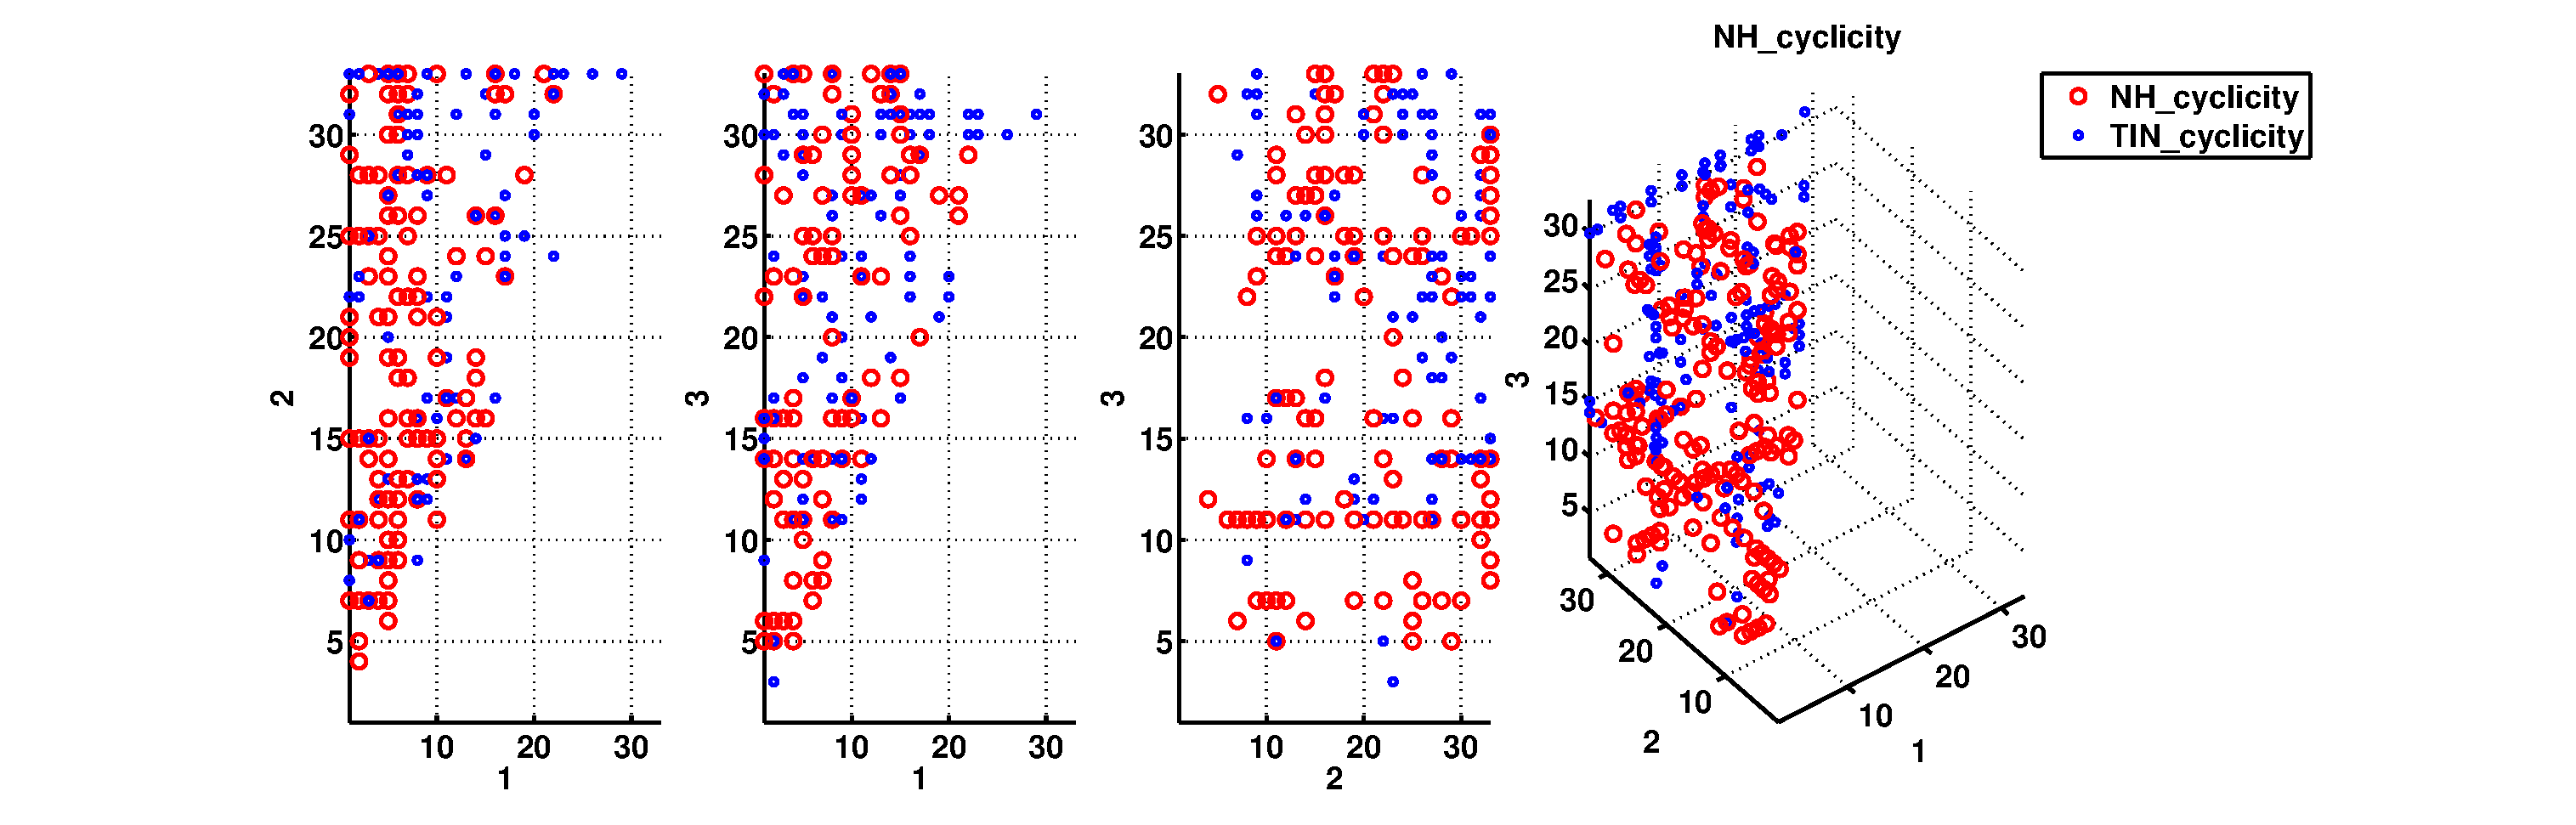
\includegraphics[width=\linewidth]{figs/makeTriples.eps}
\end{minipage}
\caption{Visual representation of triples comparing common triples in different groups. The plots show a marker wherever there is a triple for each group.}
\label{fig:makeTriples}
\end{figure}

In addition to the plots, we used the saved results with some additional processing to analyze and compare the results. This is more or less where we left off. 

\end{document}